\documentclass{article}\usepackage[]{graphicx}\usepackage[]{color}
% maxwidth is the original width if it is less than linewidth
% otherwise use linewidth (to make sure the graphics do not exceed the margin)
\makeatletter
\def\maxwidth{ %
  \ifdim\Gin@nat@width>\linewidth
    \linewidth
  \else
    \Gin@nat@width
  \fi
}
\makeatother

\definecolor{fgcolor}{rgb}{0.345, 0.345, 0.345}
\newcommand{\hlnum}[1]{\textcolor[rgb]{0.686,0.059,0.569}{#1}}%
\newcommand{\hlstr}[1]{\textcolor[rgb]{0.192,0.494,0.8}{#1}}%
\newcommand{\hlcom}[1]{\textcolor[rgb]{0.678,0.584,0.686}{\textit{#1}}}%
\newcommand{\hlopt}[1]{\textcolor[rgb]{0,0,0}{#1}}%
\newcommand{\hlstd}[1]{\textcolor[rgb]{0.345,0.345,0.345}{#1}}%
\newcommand{\hlkwa}[1]{\textcolor[rgb]{0.161,0.373,0.58}{\textbf{#1}}}%
\newcommand{\hlkwb}[1]{\textcolor[rgb]{0.69,0.353,0.396}{#1}}%
\newcommand{\hlkwc}[1]{\textcolor[rgb]{0.333,0.667,0.333}{#1}}%
\newcommand{\hlkwd}[1]{\textcolor[rgb]{0.737,0.353,0.396}{\textbf{#1}}}%
\let\hlipl\hlkwb

\usepackage{framed}
\makeatletter
\newenvironment{kframe}{%
 \def\at@end@of@kframe{}%
 \ifinner\ifhmode%
  \def\at@end@of@kframe{\end{minipage}}%
  \begin{minipage}{\columnwidth}%
 \fi\fi%
 \def\FrameCommand##1{\hskip\@totalleftmargin \hskip-\fboxsep
 \colorbox{shadecolor}{##1}\hskip-\fboxsep
     % There is no \\@totalrightmargin, so:
     \hskip-\linewidth \hskip-\@totalleftmargin \hskip\columnwidth}%
 \MakeFramed {\advance\hsize-\width
   \@totalleftmargin\z@ \linewidth\hsize
   \@setminipage}}%
 {\par\unskip\endMakeFramed%
 \at@end@of@kframe}
\makeatother

\definecolor{shadecolor}{rgb}{.97, .97, .97}
\definecolor{messagecolor}{rgb}{0, 0, 0}
\definecolor{warningcolor}{rgb}{1, 0, 1}
\definecolor{errorcolor}{rgb}{1, 0, 0}
\newenvironment{knitrout}{}{} % an empty environment to be redefined in TeX

\usepackage{alltt}
\usepackage[a4paper, total={6.5in, 8.5in}]{geometry}
\usepackage{fullpage}
\usepackage{url,hyperref}
\usepackage{graphicx}
\usepackage{amsmath,amssymb,array,comment,eucal}
\usepackage{algorithm}
\usepackage{titlesec}
\usepackage[noend]{algpseudocode}
\usepackage{enumitem}
\newlist{steps}{enumerate}{1}
\setlist[steps, 1]{label = Step \arabic*:}
\titleformat{\section}
{\normalfont\Large\bfseries}{Exercise~\thesection}{1em}{}
\newcommand\T{\textrm{T}}
\newcommand\N{\mathcal{N}}
\newcommand\bX{\mathbf{X}}
\newcommand\bx{\mathbf{x}}
\newcommand\bxm{\bar{\bx}}
\newcommand\bXtX{\mathbf{X}^T\mathbf{X}}
\newcommand\bY{\mathbf{Y}}
\newcommand\by{\mathbf{y}}
\newcommand\bI{\mathbf{I}}
\newcommand\bP{\mathbf{P}}
\newcommand\bPX{\mathbf{P}_{\bX}}
\newcommand\bU{\mathbf{U}}
\newcommand\bD{\mathbf{D}}
\newcommand\beps{\boldsymbol{\epsilon}}
\newcommand\bgamma{\boldsymbol{\gamma}}
\newcommand\one{\mathbf{1}}
\newcommand\zero{\mathbf{0}}
\newcommand\mby{\bar{\by}}
\newcommand\my{\bar{y}}
\newcommand\bYhat{\hat{\bY}}
\newcommand\bmu{\boldsymbol{\mu}}
\newcommand\btau{\boldsymbol{\tau}}
\newcommand\blambda{\boldsymbol{\lambda}}
\newcommand\bbeta{\boldsymbol{\beta}}
\newcommand\bbetahat{\hat{\bbeta}}
\newcommand\bbetag{\bbeta_{\bgamma}}
\newcommand\bbetamg{\bbeta_{1-\bgamma}}
\newcommand\bbetatilde{\tilde{\bbeta}}
\newcommand\betahat{\hat{\beta}}
\newcommand\bXg{\bX_{\bgamma}}
\newcommand\bXmg{\bX_{1-\bgamma}}
\newcommand{\norm}[1]{\left\lVert#1\right\rVert}
%\nexcommmand\Ex{\mathbb{E}}
\IfFileExists{upquote.sty}{\usepackage{upquote}}{}
\begin{document}
\title{Case Study 1 - }
\author{Alessandro Zito}
\date{\today}
\maketitle

\section*{R setup}
\begin{knitrout}
\definecolor{shadecolor}{rgb}{0.969, 0.969, 0.969}\color{fgcolor}\begin{kframe}
\begin{alltt}
\hlkwd{suppressMessages}\hlstd{(}\hlkwd{library}\hlstd{(tidyverse))}
\hlkwd{library}\hlstd{(corrplot)}
\end{alltt}


{\ttfamily\noindent\itshape\color{messagecolor}{\#\# corrplot 0.84 loaded}}\begin{alltt}
\hlkwd{library}\hlstd{(RColorBrewer)}
\hlstd{ggplot2}\hlopt{::}\hlkwd{theme_set}\hlstd{(ggplot2}\hlopt{::}\hlkwd{theme_bw}\hlstd{())}
\end{alltt}
\end{kframe}
\end{knitrout}

\section{Introduction}

\section{EDA}
We import the data and make a summary of the main values
\begin{knitrout}
\definecolor{shadecolor}{rgb}{0.969, 0.969, 0.969}\color{fgcolor}\begin{kframe}
\begin{alltt}
\hlcom{# Import the data and observe the missing values / wierd values}
\hlstd{data} \hlkwb{=} \hlkwd{readRDS}\hlstd{(}\hlstr{"Longnecker.rds"}\hlstd{)}
\hlkwd{print}\hlstd{(}\hlkwd{dim}\hlstd{(data))}
\end{alltt}
\begin{verbatim}
## [1] 2380   23
\end{verbatim}
\begin{alltt}
\hlcom{# The variables of interest are DDE, all the PBCs. }
\hlcom{# The dependent variable is gestational_age}
\end{alltt}
\end{kframe}
\end{knitrout}
The plot of gestational age is 
\begin{knitrout}
\definecolor{shadecolor}{rgb}{0.969, 0.969, 0.969}\color{fgcolor}\begin{kframe}
\begin{alltt}
\hlkwd{ggplot}\hlstd{(}\hlkwc{data} \hlstd{= data)} \hlopt{+}
  \hlkwd{geom_histogram}\hlstd{(}\hlkwd{aes}\hlstd{(}\hlkwc{x}\hlstd{=gestational_age))}
\end{alltt}


{\ttfamily\noindent\itshape\color{messagecolor}{\#\# `stat\_bin()` using `bins = 30`. Pick better value with `binwidth`.}}\end{kframe}
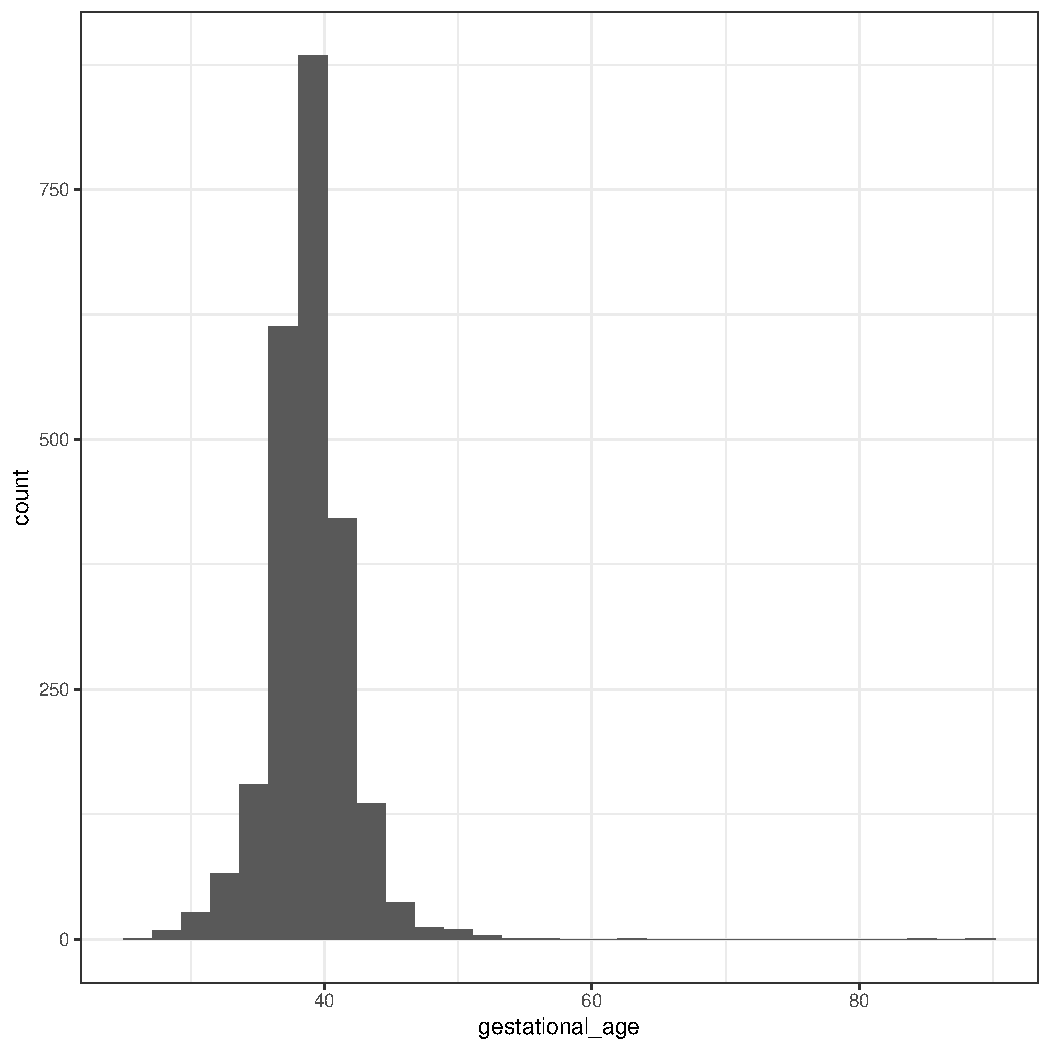
\includegraphics[width=\maxwidth]{figure/unnamed-chunk-3-1} 

\end{knitrout}
We see in particular thea there are wierd values in the dependent variable. Indeed, the highest number of weeks obsrved is 90
\begin{knitrout}
\definecolor{shadecolor}{rgb}{0.969, 0.969, 0.969}\color{fgcolor}\begin{kframe}
\begin{alltt}
\hlkwd{table}\hlstd{(data}\hlopt{$}\hlstd{gestational_age)}
\end{alltt}
\begin{verbatim}
## 
##  27  28  29  30  31  32  33  34  35  36  37  38  39  40  41  42  43  44  45  46 
##   1   4   5   8  19  32  34  67  88 103 161 349 425 459 279 142  79  57  25  12 
##  47  48  49  50  51  52  53  55  56  64  84  90 
##   8   4   4   3   3   3   1   1   1   1   1   1
\end{verbatim}
\end{kframe}
\end{knitrout}
As the record for longest pregnancy in weeks is equal to 375 and the second one is 317, we decide to drop all the observations which have a gestational age higher than 46 weeks (excluded). Moreoer, we transform smoking stauts and center as factors and we drop albumin (which is only made by NAs). Finally, we create a variable that reports if the the birth has been premature or not (before 37 weeks). 
\begin{knitrout}
\definecolor{shadecolor}{rgb}{0.969, 0.969, 0.969}\color{fgcolor}\begin{kframe}
\begin{alltt}
\hlstd{data} \hlkwb{=} \hlstd{data} \hlopt
  \hlkwd{filter}\hlstd{(gestational_age} \hlopt{<=} \hlnum{46}\hlstd{)} \hlopt
  \hlkwd{mutate_at}\hlstd{(}\hlkwd{vars}\hlstd{(smoking_status, center),factor)} \hlopt
  \hlkwd{select}\hlstd{(}\hlopt{-}\hlstd{albumin)} \hlopt \hlcom{#Too many NAs}
  \hlkwd{mutate}\hlstd{(}\hlkwc{premature} \hlstd{= (gestational_age} \hlopt{<} \hlnum{37}\hlstd{))}
\end{alltt}
\end{kframe}
\end{knitrout}
We start by exploiting the relationship between the new variable premature and the DDE. Note that the number of premature mothers compared to the size of the new dataset is
\begin{knitrout}
\definecolor{shadecolor}{rgb}{0.969, 0.969, 0.969}\color{fgcolor}\begin{kframe}
\begin{alltt}
\hlkwd{table}\hlstd{(data}\hlopt{$}\hlstd{premature)}
\end{alltt}
\begin{verbatim}
## 
## FALSE  TRUE 
##  1988   361
\end{verbatim}
\begin{alltt}
\hlkwd{table}\hlstd{(data}\hlopt{$}\hlstd{premature)}\hlopt{/}\hlkwd{nrow}\hlstd{(data)}
\end{alltt}
\begin{verbatim}
## 
##     FALSE      TRUE 
## 0.8463176 0.1536824
\end{verbatim}
\end{kframe}
\end{knitrout}
and the association it has with DDE is positive. 
\begin{knitrout}
\definecolor{shadecolor}{rgb}{0.969, 0.969, 0.969}\color{fgcolor}\begin{kframe}
\begin{alltt}
\hlkwd{ggplot}\hlstd{(data)} \hlopt{+}
  \hlkwd{geom_boxplot}\hlstd{(}\hlkwd{aes}\hlstd{(}\hlkwc{x}\hlstd{=premature,} \hlkwc{y}\hlstd{=dde))}
\end{alltt}
\end{kframe}
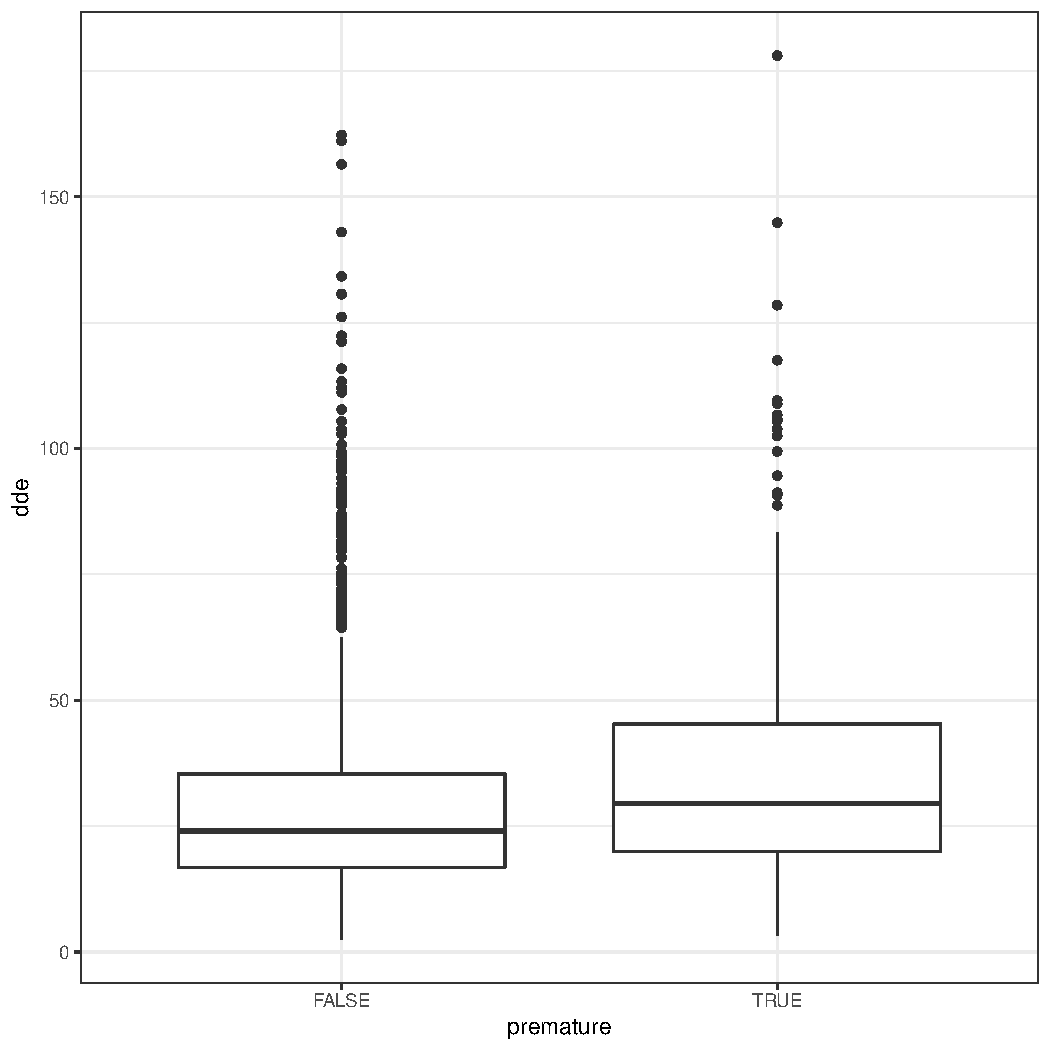
\includegraphics[width=\maxwidth]{figure/unnamed-chunk-7-1} 

\end{knitrout}
To see the relationship between premature and pcb, we have to understand what is the correlation across each level of pcb. Notice that there is only one row that has null values ofr pcb. We decide to drop it.
\begin{knitrout}
\definecolor{shadecolor}{rgb}{0.969, 0.969, 0.969}\color{fgcolor}\begin{kframe}
\begin{alltt}
\hlstd{data} \hlkwb{=} \hlstd{data[}\hlopt{-}\hlkwd{is.na}\hlstd{(data}\hlopt{$}\hlstd{pcb_028),]}
\end{alltt}
\end{kframe}
\end{knitrout}
\begin{knitrout}
\definecolor{shadecolor}{rgb}{0.969, 0.969, 0.969}\color{fgcolor}\begin{kframe}
\begin{alltt}
\hlstd{cor_base} \hlkwb{=} \hlkwd{cor}\hlstd{(data} \hlopt \hlkwd{select}\hlstd{(}\hlopt{-}\hlstd{smoking_status,} \hlopt{-}\hlstd{race,} \hlopt{-}\hlstd{center,} \hlopt{-}\hlstd{premature),} \hlkwc{use}\hlstd{=}\hlstr{"pairwise.complete.obs"} \hlstd{)}
\hlkwd{corrplot}\hlstd{(cor_base,}\hlkwc{col}\hlstd{=}\hlkwd{brewer.pal}\hlstd{(}\hlkwc{n}\hlstd{=}\hlnum{8}\hlstd{,} \hlkwc{name}\hlstd{=}\hlstr{"RdYlBu"}\hlstd{))}
\end{alltt}
\end{kframe}
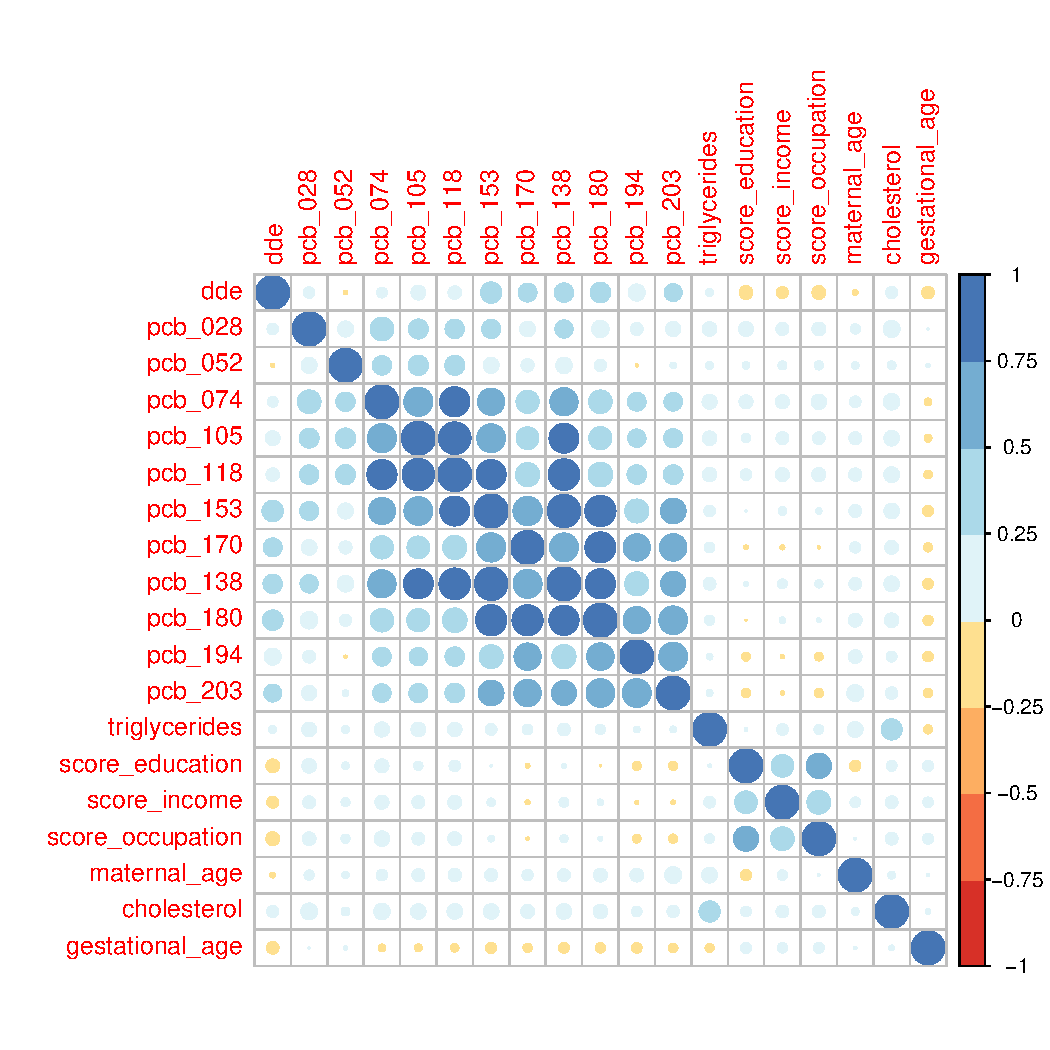
\includegraphics[width=\maxwidth]{figure/unnamed-chunk-9-1} 

\end{knitrout}
We see that each pcb are very correlated among themselves. This is expected, as they originate from one single component. As the variables have their own unit of measure, we suggest two approaches.  
\begin{enumerate}
\item Summing them (to see the total amount of pcb in the blood).
\item Standardizing and averaging them
\end{enumerate}
\begin{knitrout}
\definecolor{shadecolor}{rgb}{0.969, 0.969, 0.969}\color{fgcolor}\begin{kframe}
\begin{alltt}
\hlcom{# 1) Summing}
\hlstd{pcb_sum} \hlkwb{=} \hlkwd{apply}\hlstd{(}\hlkwd{as.matrix}\hlstd{(data} \hlopt \hlkwd{select}\hlstd{(pcb_028, pcb_052, pcb_074, pcb_105, pcb_118, pcb_153, pcb_170, pcb_138, pcb_180, pcb_194, pcb_203)),}\hlnum{1}\hlstd{, sum)}
\hlcom{# 2) Stanardize and average}
\hlstd{my_standardize} \hlkwb{<-} \hlkwa{function}\hlstd{(}\hlkwc{x}\hlstd{) (x} \hlopt{-} \hlkwd{mean}\hlstd{(x,} \hlkwc{na.rm} \hlstd{= T))} \hlopt{/} \hlkwd{sd}\hlstd{(x,} \hlkwc{na.rm} \hlstd{= T)}
\hlstd{data} \hlkwb{=} \hlstd{data} \hlopt
  \hlkwd{mutate_at}\hlstd{(}\hlkwd{vars}\hlstd{(}\hlkwd{starts_with}\hlstd{(}\hlstr{"pcb"}\hlstd{)), my_standardize)} \hlopt \hlcom{# standardize pcb's to give them all equal weight in the aggregate pcb variable}
  \hlkwd{rowwise}\hlstd{()} \hlopt
  \hlkwd{mutate}\hlstd{(}\hlkwc{pcb_mean} \hlstd{=} \hlkwd{mean}\hlstd{(}\hlkwd{c}\hlstd{(pcb_028, pcb_052, pcb_074, pcb_105, pcb_118, pcb_153, pcb_170, pcb_138, pcb_180, pcb_194, pcb_203)))} \hlopt
  \hlstd{ungroup}
\hlstd{data}\hlopt{$}\hlstd{pcb_sum} \hlkwb{=} \hlstd{pcb_sum}
\end{alltt}
\end{kframe}
\end{knitrout}
Thus, we can mirror the boxplot with DDE and premature also in this case.
\begin{knitrout}
\definecolor{shadecolor}{rgb}{0.969, 0.969, 0.969}\color{fgcolor}\begin{kframe}
\begin{alltt}
\hlkwd{ggplot}\hlstd{(data)} \hlopt{+}
  \hlkwd{geom_boxplot}\hlstd{(}\hlkwd{aes}\hlstd{(}\hlkwc{x}\hlstd{=premature,} \hlkwc{y}\hlstd{= pcb_mean))}
\end{alltt}


{\ttfamily\noindent\color{warningcolor}{\#\# Warning: Removed 1 rows containing non-finite values (stat\_boxplot).}}\end{kframe}
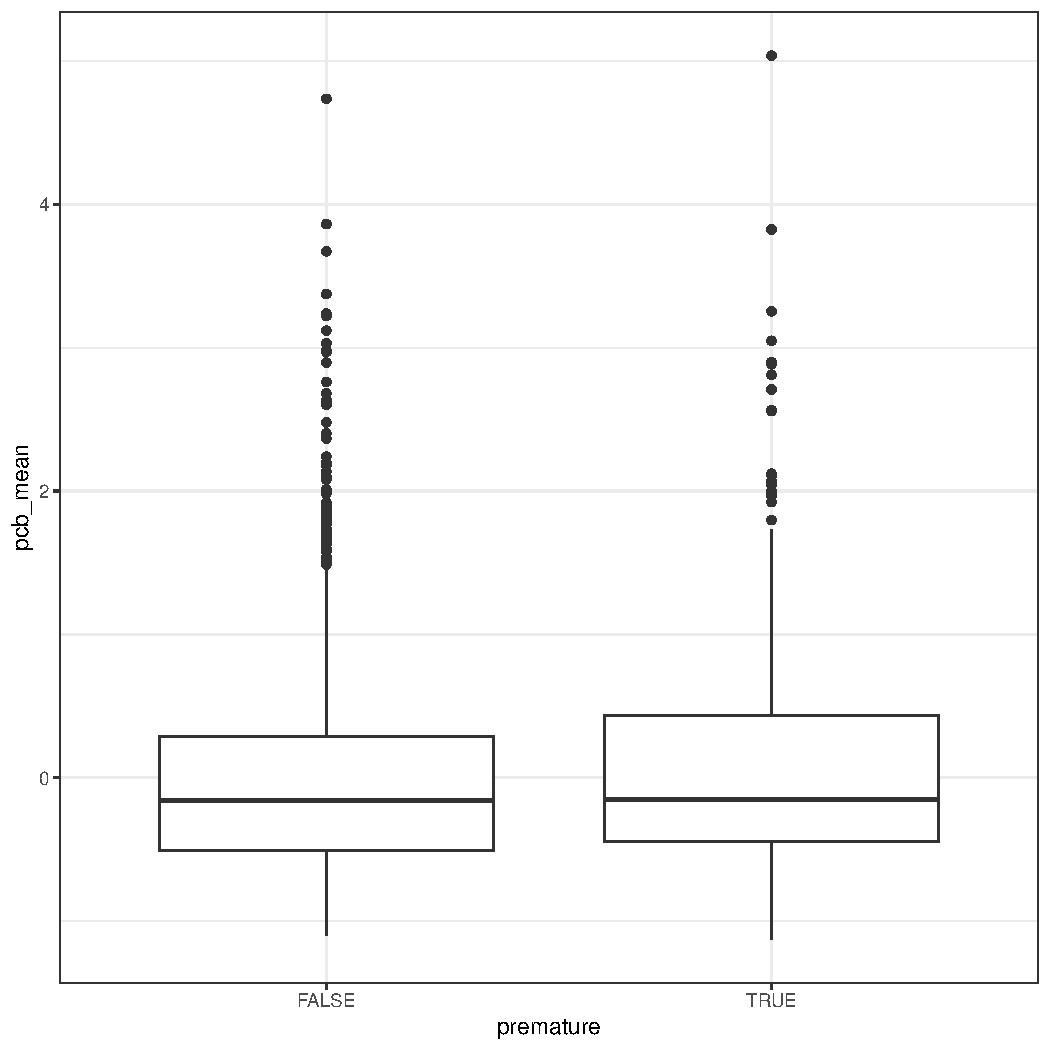
\includegraphics[width=\maxwidth]{figure/unnamed-chunk-11-1} 
\begin{kframe}\begin{alltt}
\hlkwd{ggplot}\hlstd{(data)} \hlopt{+}
  \hlkwd{geom_boxplot}\hlstd{(}\hlkwd{aes}\hlstd{(}\hlkwc{x}\hlstd{=premature,} \hlkwc{y}\hlstd{= pcb_sum))}
\end{alltt}


{\ttfamily\noindent\color{warningcolor}{\#\# Warning: Removed 1 rows containing non-finite values (stat\_boxplot).}}\end{kframe}
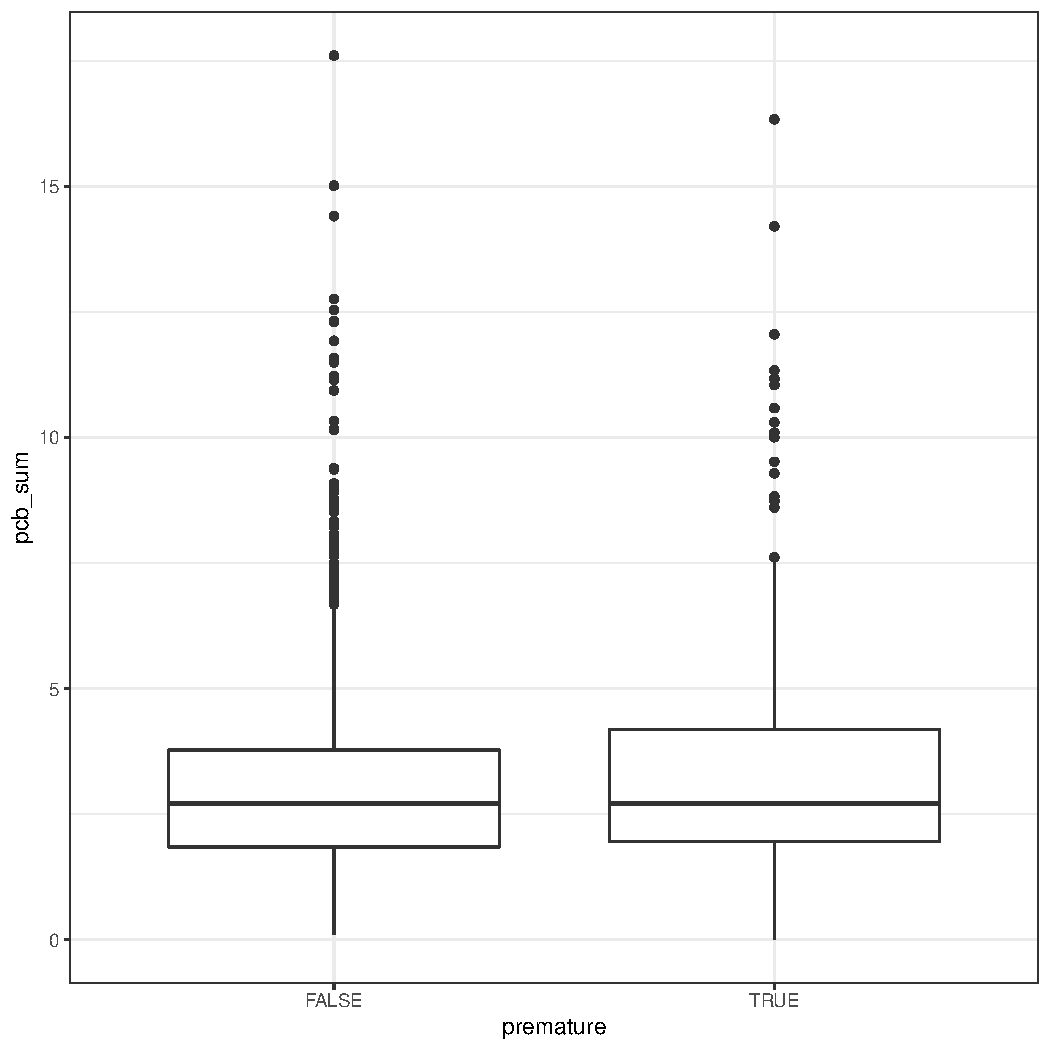
\includegraphics[width=\maxwidth]{figure/unnamed-chunk-11-2} 

\end{knitrout}
We see that the results are very similar. This suggests that the approaches will lead to the same results. 
At last, we isolate the results between environment and not environment (as raphael suggested). 
\begin{knitrout}
\definecolor{shadecolor}{rgb}{0.969, 0.969, 0.969}\color{fgcolor}\begin{kframe}
\begin{alltt}
\hlkwd{cor}\hlstd{(data} \hlopt \hlkwd{select}\hlstd{(triglycerides, cholesterol))}
\end{alltt}
\begin{verbatim}
##               triglycerides cholesterol
## triglycerides     1.0000000   0.3610952
## cholesterol       0.3610952   1.0000000
\end{verbatim}
\begin{alltt}
\hlstd{data} \hlkwb{=} \hlstd{data} \hlopt \hlkwd{rowwise}\hlstd{()} \hlopt \hlkwd{mutate}\hlstd{(}\hlkwc{trigl_chol_sum} \hlstd{=} \hlkwd{sum}\hlstd{(triglycerides, cholesterol))} \hlopt \hlstd{ungroup}
\hlstd{data}\hlopt{$}\hlstd{dde_env} \hlkwb{=} \hlstd{data}\hlopt{$}\hlstd{dde}\hlopt{/}\hlstd{data}\hlopt{$}\hlstd{trigl_chol_sum}
\hlstd{data}\hlopt{$}\hlstd{pcb_sum_env} \hlkwb{=} \hlstd{data}\hlopt{$}\hlstd{pcb_sum}\hlopt{/}\hlstd{data}\hlopt{$}\hlstd{trigl_chol_sum}
\hlkwd{ggplot}\hlstd{(data)} \hlopt{+}
  \hlkwd{geom_boxplot}\hlstd{(}\hlkwd{aes}\hlstd{(}\hlkwc{x}\hlstd{=premature,} \hlkwc{y}\hlstd{= pcb_sum_env))}
\end{alltt}


{\ttfamily\noindent\color{warningcolor}{\#\# Warning: Removed 1 rows containing non-finite values (stat\_boxplot).}}\end{kframe}
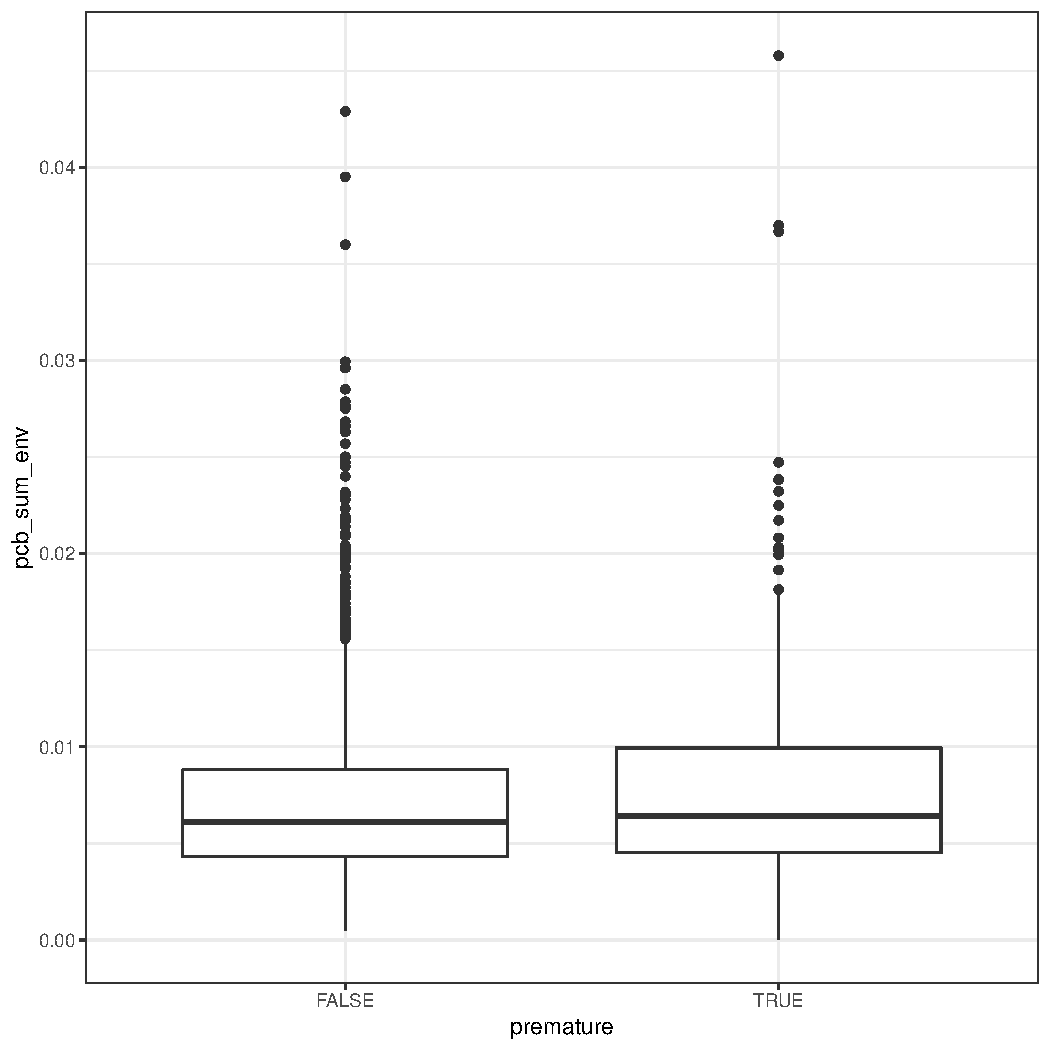
\includegraphics[width=\maxwidth]{figure/unnamed-chunk-12-1} 

\end{knitrout}
\begin{knitrout}
\definecolor{shadecolor}{rgb}{0.969, 0.969, 0.969}\color{fgcolor}\begin{kframe}
\begin{alltt}
\hlcom{# use the formula in Roberts et al}
\hlstd{data}\hlopt{$}\hlstd{lipids} \hlkwb{=} \hlnum{2.27}\hlopt{*}\hlstd{data}\hlopt{$}\hlstd{cholesterol} \hlopt{+}  \hlstd{data}\hlopt{$}\hlstd{triglycerides} \hlopt{+} \hlnum{0.623}
\hlstd{data}\hlopt{$}\hlstd{dde_lipid} \hlkwb{=} \hlstd{data}\hlopt{$}\hlstd{dde}\hlopt{/}\hlstd{data}\hlopt{$}\hlstd{lipids}
\hlstd{data}\hlopt{$}\hlstd{pcb_lipid} \hlkwb{=} \hlstd{data}\hlopt{$}\hlstd{pcb_sum}\hlopt{/}\hlstd{data}\hlopt{$}\hlstd{lipids}
\end{alltt}
\end{kframe}
\end{knitrout}

One last thing. How are the premature women distributed across the centers?
\begin{knitrout}
\definecolor{shadecolor}{rgb}{0.969, 0.969, 0.969}\color{fgcolor}\begin{kframe}
\begin{alltt}
\hlstd{data}\hlopt{$}\hlstd{premature} \hlkwb{=} \hlkwd{as.numeric}\hlstd{(data}\hlopt{$}\hlstd{premature)}
\hlkwd{barplot}\hlstd{(}\hlkwd{table}\hlstd{(data}\hlopt{$}\hlstd{premature, data}\hlopt{$}\hlstd{center))}
\end{alltt}
\end{kframe}
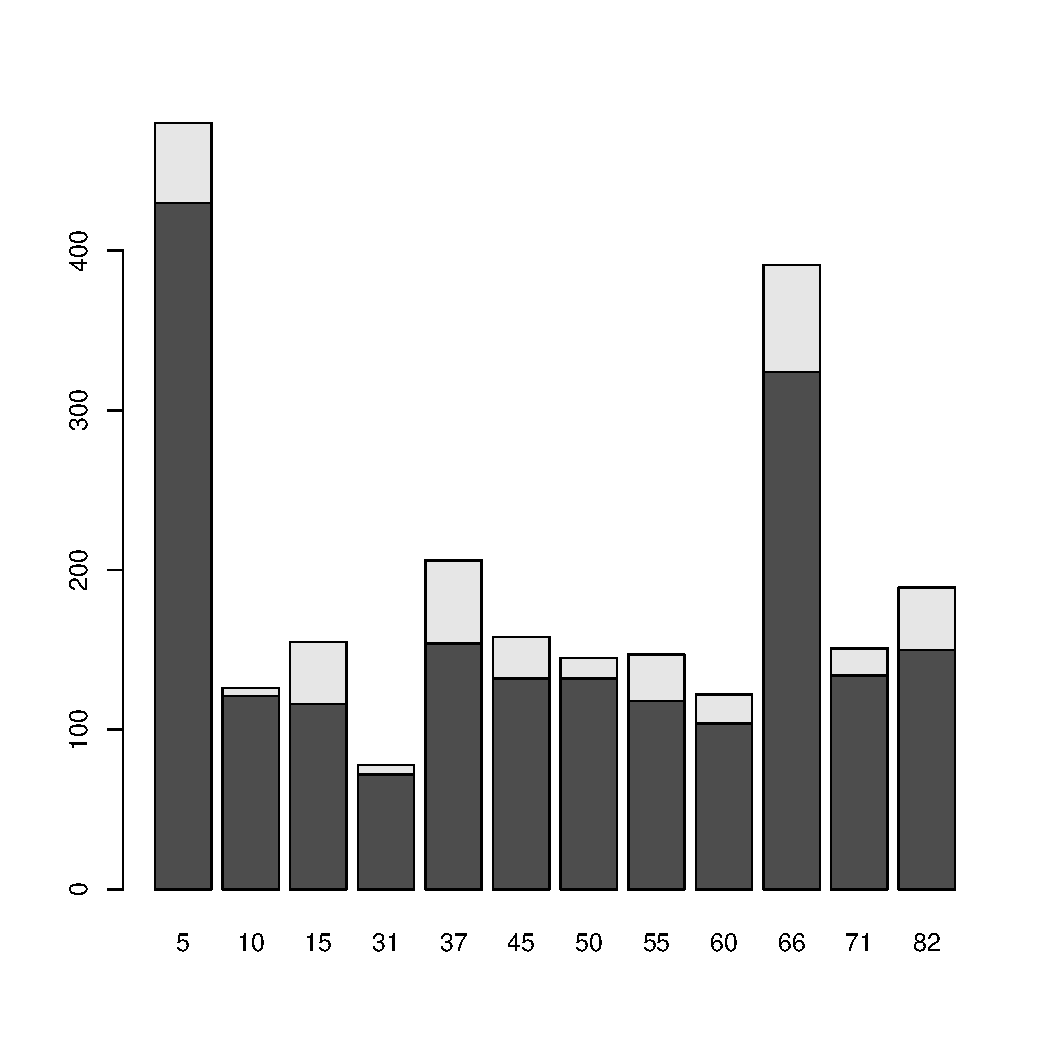
\includegraphics[width=\maxwidth]{figure/unnamed-chunk-14-1} 
\begin{kframe}\begin{alltt}
\hlstd{data} \hlopt
  \hlkwd{ggplot}\hlstd{(}\hlkwd{aes}\hlstd{(}\hlkwc{x}\hlstd{=center,} \hlkwc{fill} \hlstd{=} \hlkwd{as.factor}\hlstd{(premature)))} \hlopt{+}
  \hlkwd{geom_bar}\hlstd{(}\hlkwc{position} \hlstd{=} \hlstr{"fill"}\hlstd{)}
\end{alltt}
\end{kframe}
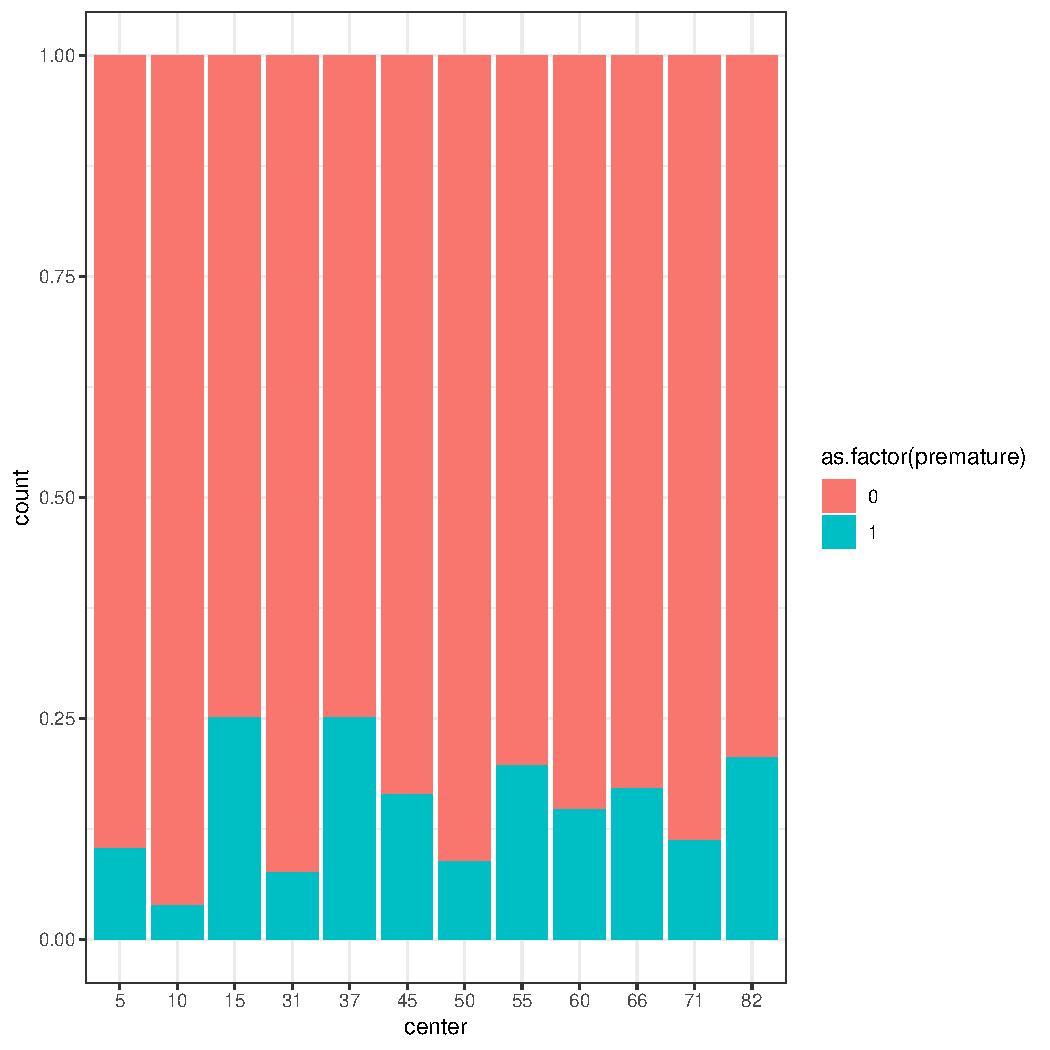
\includegraphics[width=\maxwidth]{figure/unnamed-chunk-14-2} 

\end{knitrout}
From a first glance,the labs seem eterogeneous. This is a problem we need to deal with. 

\section{A first approach: logistic regression}
We run a very simple logistic regression. First, we focus on the complete cases (to add all regressors). We start in the simple case of the dde and pcb\_sum without the environment effect.
\begin{knitrout}
\definecolor{shadecolor}{rgb}{0.969, 0.969, 0.969}\color{fgcolor}\begin{kframe}
\begin{alltt}
\hlstd{logit_model_1} \hlkwb{<-} \hlkwd{glm}\hlstd{(premature} \hlopt{~} \hlstd{dde} \hlopt{+} \hlstd{pcb_sum} \hlopt{+} \hlstd{race} \hlopt{+} \hlstd{maternal_age} \hlopt{+} \hlstd{score_occupation} \hlopt{+} \hlstd{center} \hlopt{+} \hlstd{score_income} \hlopt{+} \hlstd{score_education,} \hlkwc{data} \hlstd{= data,} \hlkwc{family} \hlstd{=} \hlstr{"binomial"}\hlstd{)}
\hlkwd{summary}\hlstd{(logit_model_1)}
\end{alltt}
\begin{verbatim}
## 
## Call:
## glm(formula = premature ~ dde + pcb_sum + race + maternal_age + 
##     score_occupation + center + score_income + score_education, 
##     family = "binomial", data = data)
## 
## Deviance Residuals: 
##     Min       1Q   Median       3Q      Max  
## -1.3080  -0.6143  -0.4804  -0.3578   2.7137  
## 
## Coefficients:
##                   Estimate Std. Error z value Pr(>|z|)    
## (Intercept)      -2.116247   0.421263  -5.024 5.07e-07 ***
## dde               0.009322   0.003254   2.865  0.00417 ** 
## pcb_sum           0.107112   0.039410   2.718  0.00657 ** 
## raceblack         0.258101   0.241582   1.068  0.28535    
## raceother         0.803932   0.494812   1.625  0.10422    
## maternal_age     -0.004595   0.011105  -0.414  0.67906    
## score_occupation -0.003767   0.002830  -1.331  0.18322    
## center10         -0.870941   0.495521  -1.758  0.07881 .  
## center15          0.580670   0.371618   1.563  0.11816    
## center31         -1.003980   0.592436  -1.695  0.09014 .  
## center37          0.652792   0.303428   2.151  0.03145 *  
## center45         -0.028248   0.357586  -0.079  0.93704    
## center50          0.032301   0.367842   0.088  0.93003    
## center55         -0.448572   0.599546  -0.748  0.45435    
## center60          0.251547   0.366731   0.686  0.49276    
## center66          0.024323   0.314908   0.077  0.93843    
## center71         -0.137112   0.362607  -0.378  0.70533    
## center82          0.325151   0.367403   0.885  0.37616    
## score_income     -0.002296   0.002782  -0.825  0.40934    
## score_education  -0.004091   0.003124  -1.310  0.19036    
## ---
## Signif. codes:  0 '***' 0.001 '**' 0.01 '*' 0.05 '.' 0.1 ' ' 1
## 
## (Dispersion parameter for binomial family taken to be 1)
## 
##     Null deviance: 1549.5  on 1831  degrees of freedom
## Residual deviance: 1453.4  on 1812  degrees of freedom
##   (516 observations deleted due to missingness)
## AIC: 1493.4
## 
## Number of Fisher Scoring iterations: 5
\end{verbatim}
\end{kframe}
\end{knitrout}

\begin{knitrout}
\definecolor{shadecolor}{rgb}{0.969, 0.969, 0.969}\color{fgcolor}\begin{kframe}
\begin{alltt}
\hlstd{logit_model_2} \hlkwb{<-} \hlkwd{glm}\hlstd{(premature} \hlopt{~} \hlstd{dde_env} \hlopt{+} \hlstd{pcb_sum_env} \hlopt{+} \hlstd{race} \hlopt{+} \hlstd{maternal_age} \hlopt{+} \hlstd{score_occupation} \hlopt{+} \hlstd{center} \hlopt{+} \hlstd{score_income} \hlopt{+} \hlstd{score_education,} \hlkwc{data} \hlstd{= data,} \hlkwc{family} \hlstd{=} \hlstr{"binomial"}\hlstd{)}
\hlkwd{summary}\hlstd{(logit_model_2)}
\end{alltt}
\begin{verbatim}
## 
## Call:
## glm(formula = premature ~ dde_env + pcb_sum_env + race + maternal_age + 
##     score_occupation + center + score_income + score_education, 
##     family = "binomial", data = data)
## 
## Deviance Residuals: 
##     Min       1Q   Median       3Q      Max  
## -1.0686  -0.6225  -0.4909  -0.3649   2.6527  
## 
## Coefficients:
##                   Estimate Std. Error z value Pr(>|z|)    
## (Intercept)      -1.922867   0.418335  -4.596  4.3e-06 ***
## dde_env           3.042856   1.353676   2.248   0.0246 *  
## pcb_sum_env      20.220561  16.410417   1.232   0.2179    
## raceblack         0.279208   0.244582   1.142   0.2536    
## raceother         0.719970   0.491241   1.466   0.1428    
## maternal_age      0.000080   0.011020   0.007   0.9942    
## score_occupation -0.003359   0.002816  -1.193   0.2330    
## center10         -0.821461   0.492568  -1.668   0.0954 .  
## center15          0.431834   0.368169   1.173   0.2408    
## center31         -0.971114   0.587981  -1.652   0.0986 .  
## center37          0.607774   0.302309   2.010   0.0444 *  
## center45         -0.029969   0.354556  -0.085   0.9326    
## center50         -0.094126   0.364143  -0.258   0.7960    
## center55         -0.507646   0.593630  -0.855   0.3925    
## center60          0.129617   0.363120   0.357   0.7211    
## center66         -0.019042   0.312753  -0.061   0.9515    
## center71         -0.195226   0.360729  -0.541   0.5884    
## center82          0.191025   0.365205   0.523   0.6009    
## score_income     -0.002060   0.002756  -0.748   0.4547    
## score_education  -0.004532   0.003105  -1.460   0.1444    
## ---
## Signif. codes:  0 '***' 0.001 '**' 0.01 '*' 0.05 '.' 0.1 ' ' 1
## 
## (Dispersion parameter for binomial family taken to be 1)
## 
##     Null deviance: 1549.5  on 1831  degrees of freedom
## Residual deviance: 1466.5  on 1812  degrees of freedom
##   (516 observations deleted due to missingness)
## AIC: 1506.5
## 
## Number of Fisher Scoring iterations: 5
\end{verbatim}
\end{kframe}
\end{knitrout}

Very important way to compute the total fat
 %https://www.ncbi.nlm.nih.gov/pmc/articles/PMC3893492/

\begin{knitrout}
\definecolor{shadecolor}{rgb}{0.969, 0.969, 0.969}\color{fgcolor}\begin{kframe}
\begin{alltt}
\hlstd{logit_model_3} \hlkwb{<-} \hlkwd{glm}\hlstd{(premature} \hlopt{~} \hlstd{dde_lipid} \hlopt{+} \hlstd{pcb_lipid} \hlopt{+} \hlstd{race} \hlopt{+} \hlstd{maternal_age} \hlopt{+} \hlstd{score_occupation} \hlopt{+} \hlstd{center} \hlopt{+} \hlstd{score_income} \hlopt{+} \hlstd{score_education,} \hlkwc{data} \hlstd{= data,} \hlkwc{family} \hlstd{=} \hlstr{"binomial"}\hlstd{)}
\hlkwd{summary}\hlstd{(logit_model_3)}
\end{alltt}
\begin{verbatim}
## 
## Call:
## glm(formula = premature ~ dde_lipid + pcb_lipid + race + maternal_age + 
##     score_occupation + center + score_income + score_education, 
##     family = "binomial", data = data)
## 
## Deviance Residuals: 
##     Min       1Q   Median       3Q      Max  
## -1.0697  -0.6216  -0.4880  -0.3629   2.6690  
## 
## Coefficients:
##                   Estimate Std. Error z value Pr(>|z|)    
## (Intercept)      -1.951086   0.418108  -4.666 3.06e-06 ***
## dde_lipid         5.514664   2.290843   2.407   0.0161 *  
## pcb_lipid        41.859184  27.536098   1.520   0.1285    
## raceblack         0.262935   0.244314   1.076   0.2818    
## raceother         0.717142   0.491548   1.459   0.1446    
## maternal_age     -0.001022   0.011056  -0.092   0.9264    
## score_occupation -0.003366   0.002819  -1.194   0.2325    
## center10         -0.828758   0.492937  -1.681   0.0927 .  
## center15          0.460702   0.368586   1.250   0.2113    
## center31         -0.954794   0.588733  -1.622   0.1049    
## center37          0.610419   0.302622   2.017   0.0437 *  
## center45         -0.025858   0.354907  -0.073   0.9419    
## center50         -0.079882   0.364435  -0.219   0.8265    
## center55         -0.488912   0.593984  -0.823   0.4104    
## center60          0.143962   0.363680   0.396   0.6922    
## center66         -0.014582   0.313227  -0.047   0.9629    
## center71         -0.190828   0.360896  -0.529   0.5970    
## center82          0.206130   0.365694   0.564   0.5730    
## score_income     -0.002059   0.002759  -0.746   0.4556    
## score_education  -0.004466   0.003106  -1.438   0.1505    
## ---
## Signif. codes:  0 '***' 0.001 '**' 0.01 '*' 0.05 '.' 0.1 ' ' 1
## 
## (Dispersion parameter for binomial family taken to be 1)
## 
##     Null deviance: 1549.5  on 1831  degrees of freedom
## Residual deviance: 1464.2  on 1812  degrees of freedom
##   (516 observations deleted due to missingness)
## AIC: 1504.2
## 
## Number of Fisher Scoring iterations: 5
\end{verbatim}
\end{kframe}
\end{knitrout}

\section{}



\end{document}
